%----------------------------------------------------------------------------
%----------------------------------------------------------------------------
The resolution of the 1 m monochromator is calculated from simple assumptions. Suppose monochromatic light is incident on a rectangular slit. The far field diffraction pattern (1 m away) is collimated and sent to a diffraction grating. We assume the significant portion of the illuminated grating completely contains the central maximum of the far field diffraction pattern (squared sinc function). The angular width of the central maximum is given by
%----------------------------------------------------------------------------
\begin{equation}
\theta = 2 \arcsin \left( \frac{\lambda}{a} \right)
\end{equation}
%----------------------------------------------------------------------------
where $\lambda$ is the wavelength of the monochromatic light and $a$ is the width of the slit. Thus, the number of lines illuminated on the grating is (assuming small angles)
%----------------------------------------------------------------------------
\begin{equation}
\kappa
=
L \theta \rho
=
L 2\frac{\lambda}{a} \rho
\end{equation}
%----------------------------------------------------------------------------
where $L$ is the distance between the input slits and the collimating optic and $\rho$ is the groove density of the grating.

The resolving power $R$ of a grating monochromator can be written in terms of the number of illuminated grooves using the Rayleigh criterion \cite{Hecht:1987a}
%----------------------------------------------------------------------------
\begin{equation}
R
=
\frac
{\lambda}
{\Delta \lambda}
=
m \kappa
\label{Rayleigh}
\end{equation}
%----------------------------------------------------------------------------
where $m$ is the diffraction order. Thus
%----------------------------------------------------------------------------
\begin{equation}
\boxed{
R = 2 m L \rho \frac{\lambda}{a}.
\label{resolvance}
}
\end{equation}
%----------------------------------------------------------------------------
For the Interactive Technology CT-103 monochromator $m=1$, $L=1$ m, and $\rho=1200$ lines per mm. The grating in the CT-103 is about 3 7/8'' wide; thus there is an additional constraint on Equation \ref{resolvance}:
%----------------------------------------------------------------------------
\begin{equation}
2 \frac{\lambda}{a}L < 3\frac{7}{8}''.
\end{equation}
%----------------------------------------------------------------------------
For small slit widths (5--50 microns) figure \ref{near_GHz} (\ref{near_cm}) shows the resolution of the CT-103 calculated from Equation \ref{resolvance} for various wavelengths in GHz (inverse cm). Figures \ref{far_THz}, \ref{far_cm}, and \ref{far_nm} show the resolution of the CT-103 for larger slit widths (50--1000 microns).
%----------------------------------------------------------------------------
%----------------------------------------------------------------------------
%bb defines the bounding box for the pdf
%viewport defines the area of the pdf used
%in sidewaysfigure the last entry in bb moves the caption toward/away the pic
%in sidewaysfigure the second entry in bb moves the pic toward/away the caption
%----------------------------------------------------------------------------
\begin{figure}
\scalebox{0.8}[0.8]{
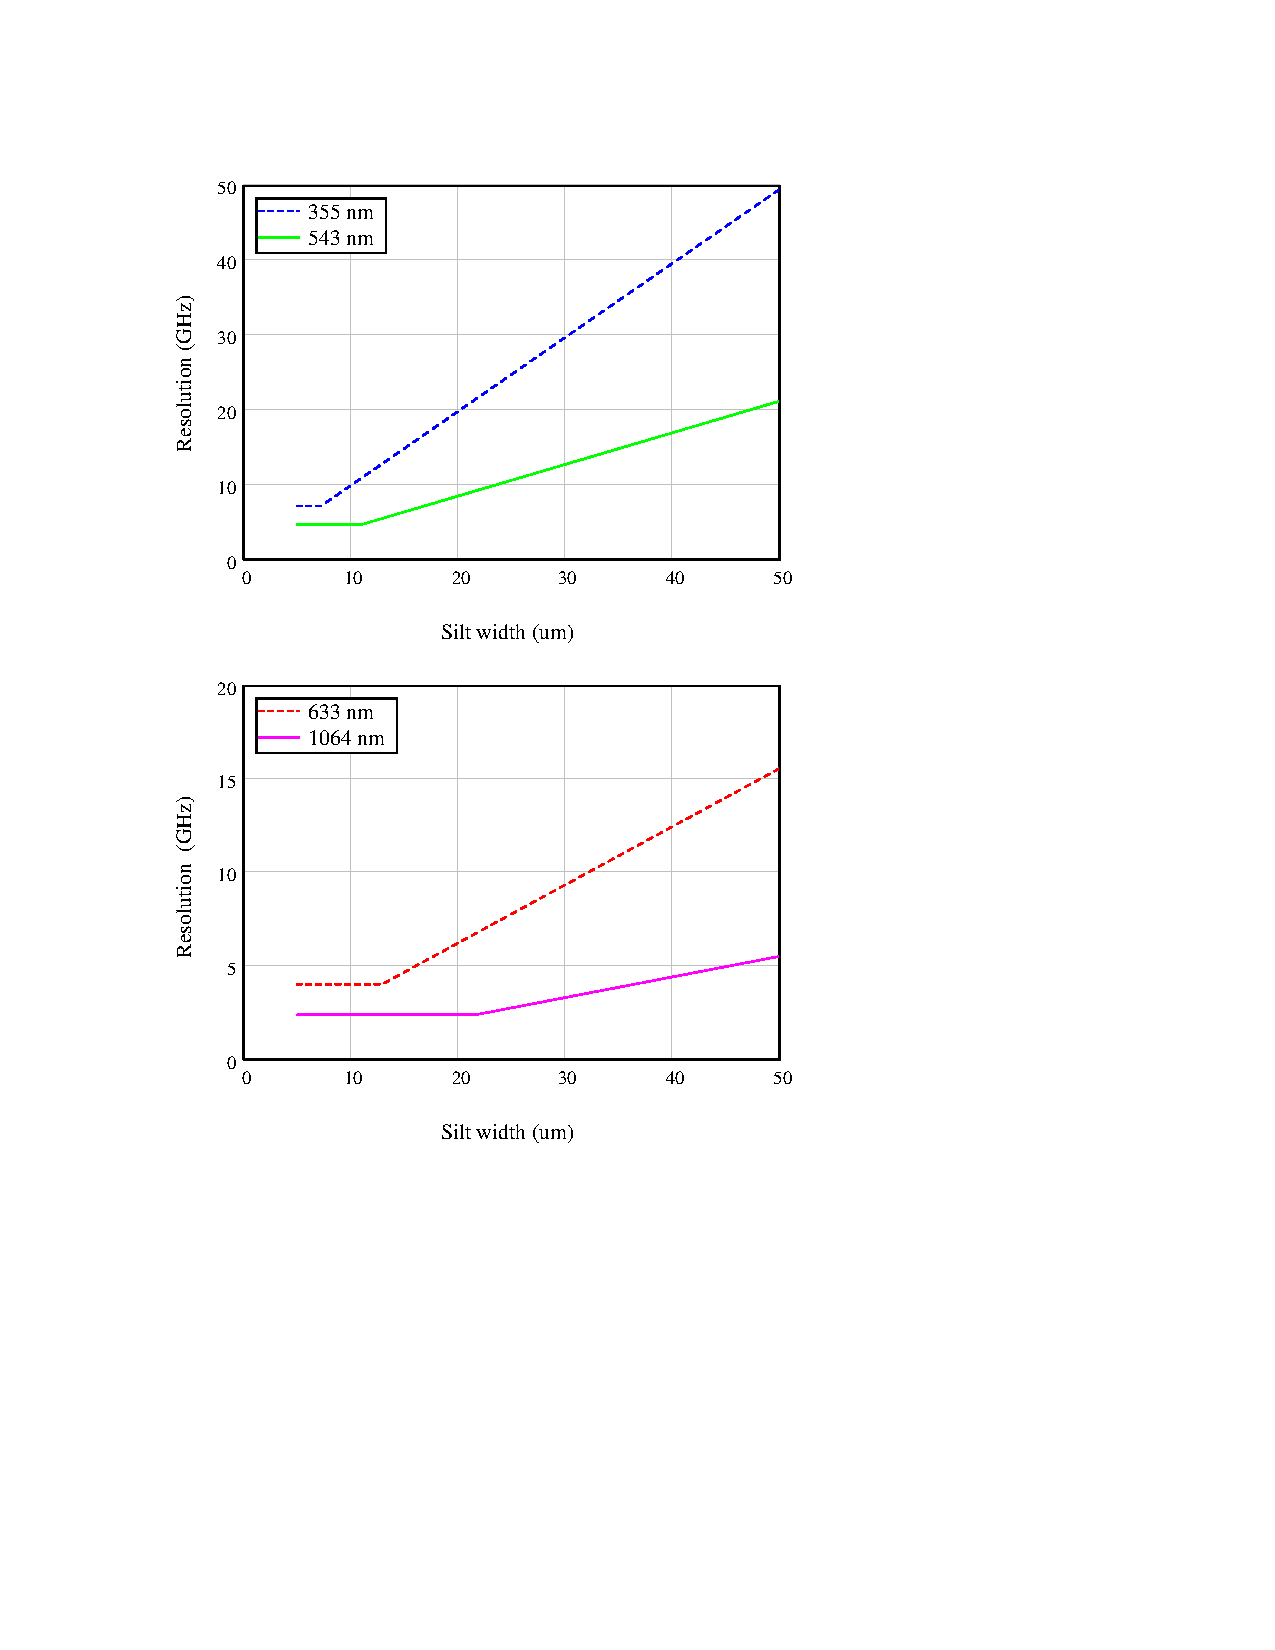
\includegraphics[bb=-30 250 489 700]
{near_GHz/near_GHz.pdf}
}
\caption{Ideal 1 m monochromator resolution (GHz)}
\label{near_GHz}
\end{figure}
%----------------------------------------------------------------------------

%----------------------------------------------------------------------------
%----------------------------------------------------------------------------
%----------------------------------------------------------------------------
%bb defines the bounding box for the pdf
%viewport defines the area of the pdf used
%in sidewaysfigure the last entry in bb moves the caption toward/away the pic
%in sidewaysfigure the second entry in bb moves the pic toward/away the caption
%----------------------------------------------------------------------------
\begin{figure}
\scalebox{0.8}[0.8]{
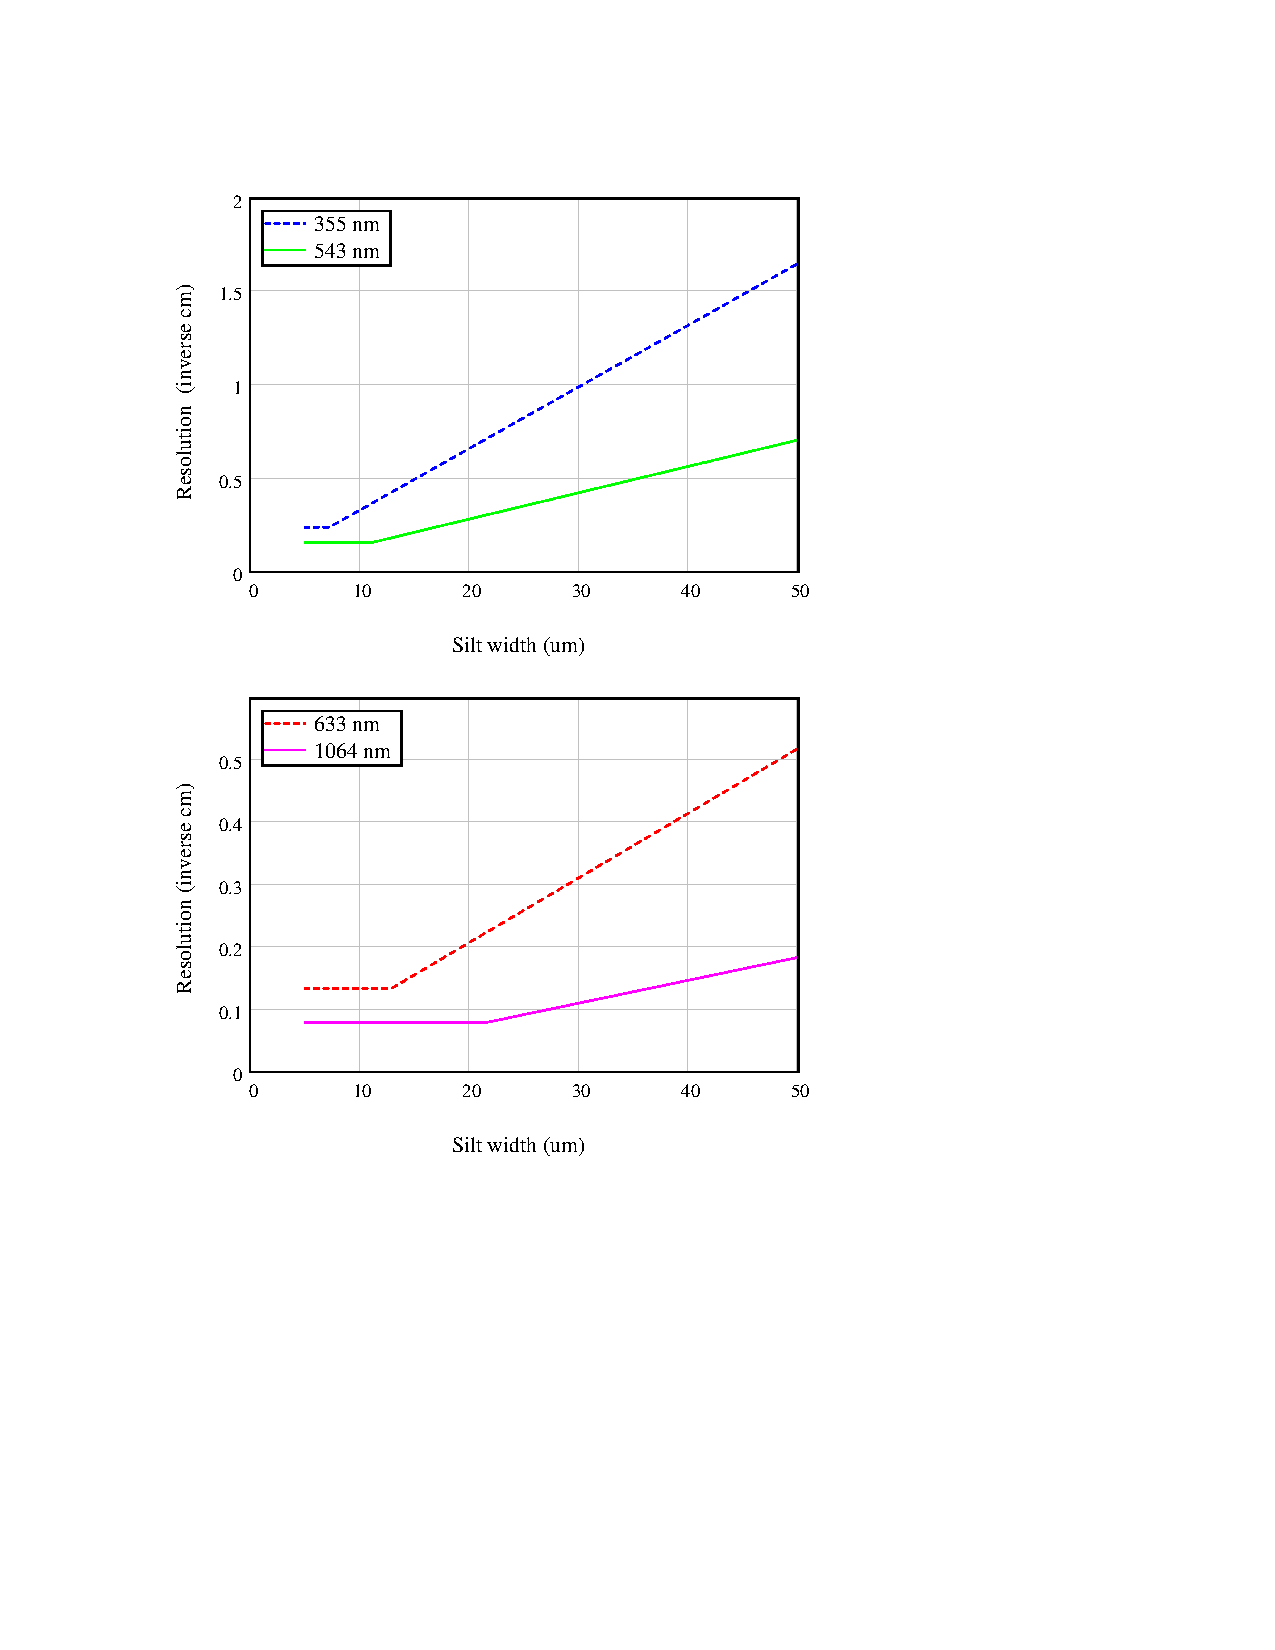
\includegraphics[bb=-30 245 489 600]
{near_cm/near_cm.pdf}
}
\caption{Ideal 1 m monochromator resolution (inverse cm)}
\label{near_cm}
\end{figure}
%----------------------------------------------------------------------------

%----------------------------------------------------------------------------
%----------------------------------------------------------------------------
%----------------------------------------------------------------------------
%bb defines the bounding box for the pdf
%viewport defines the area of the pdf used
%in sidewaysfigure the last entry in bb moves the caption toward/away the pic
%in sidewaysfigure the second entry in bb moves the pic toward/away the caption
%----------------------------------------------------------------------------
\begin{figure}
\scalebox{0.8}[0.8]{
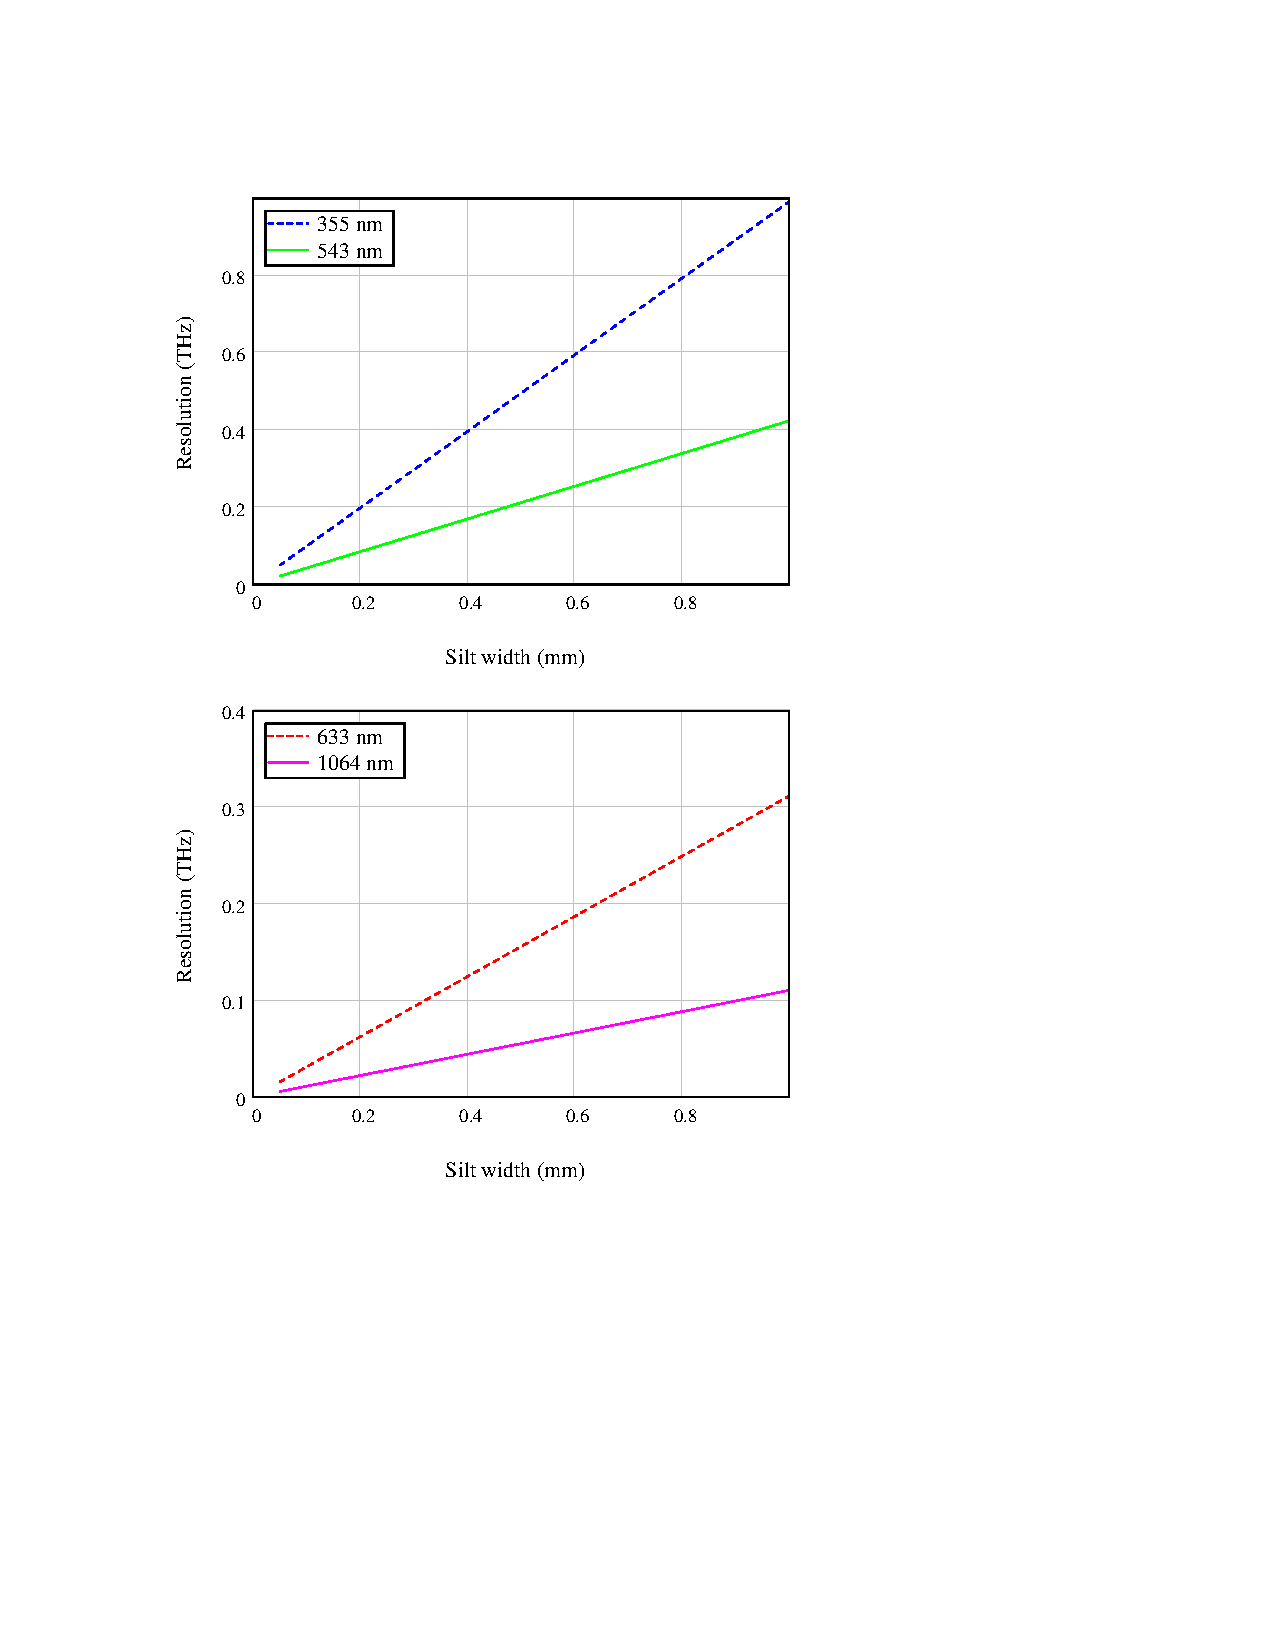
\includegraphics[bb=-30 230 489 700]
{far_THz/far_THz.pdf}
}
\caption{Ideal 1 m monochromator resolution (THz) for large slit widths}
\label{far_THz}
\end{figure}
%----------------------------------------------------------------------------

%----------------------------------------------------------------------------
%----------------------------------------------------------------------------
%----------------------------------------------------------------------------
%bb defines the bounding box for the pdf
%viewport defines the area of the pdf used
%in sidewaysfigure the last entry in bb moves the caption toward/away the pic
%in sidewaysfigure the second entry in bb moves the pic toward/away the caption
%----------------------------------------------------------------------------
\begin{figure}
\scalebox{0.8}[0.8]{
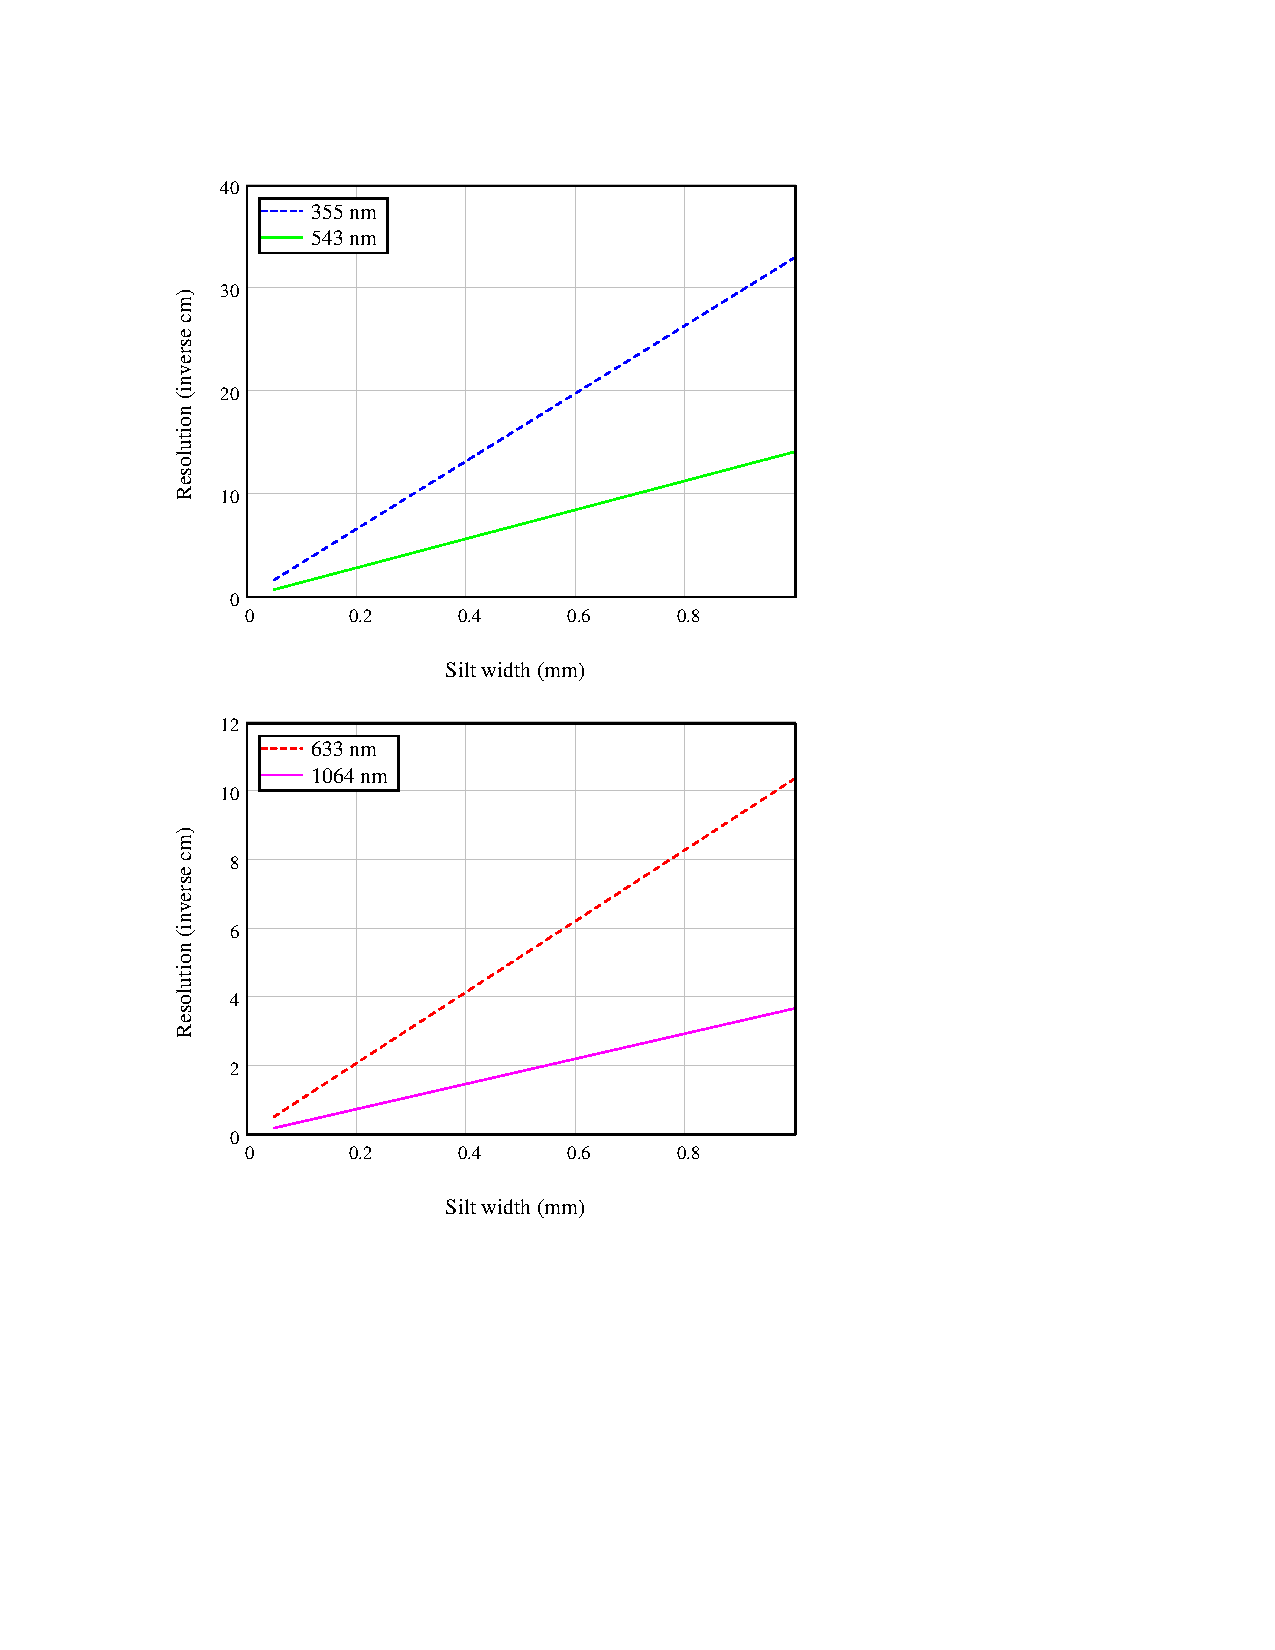
\includegraphics[bb=-30 212 489 700]
{far_cm/far_cm.pdf}
}
\caption{Ideal 1 m monochromator resolution (inverse cm) for large slit widths}
\label{far_cm}
\end{figure}
%----------------------------------------------------------------------------

%----------------------------------------------------------------------------
%----------------------------------------------------------------------------
%----------------------------------------------------------------------------
%bb defines the bounding box for the pdf
%viewport defines the area of the pdf used
%in sidewaysfigure the last entry in bb moves the caption toward/away the pic
%in sidewaysfigure the second entry in bb moves the pic toward/away the caption
%----------------------------------------------------------------------------
\begin{figure}
\scalebox{0.8}[0.8]{
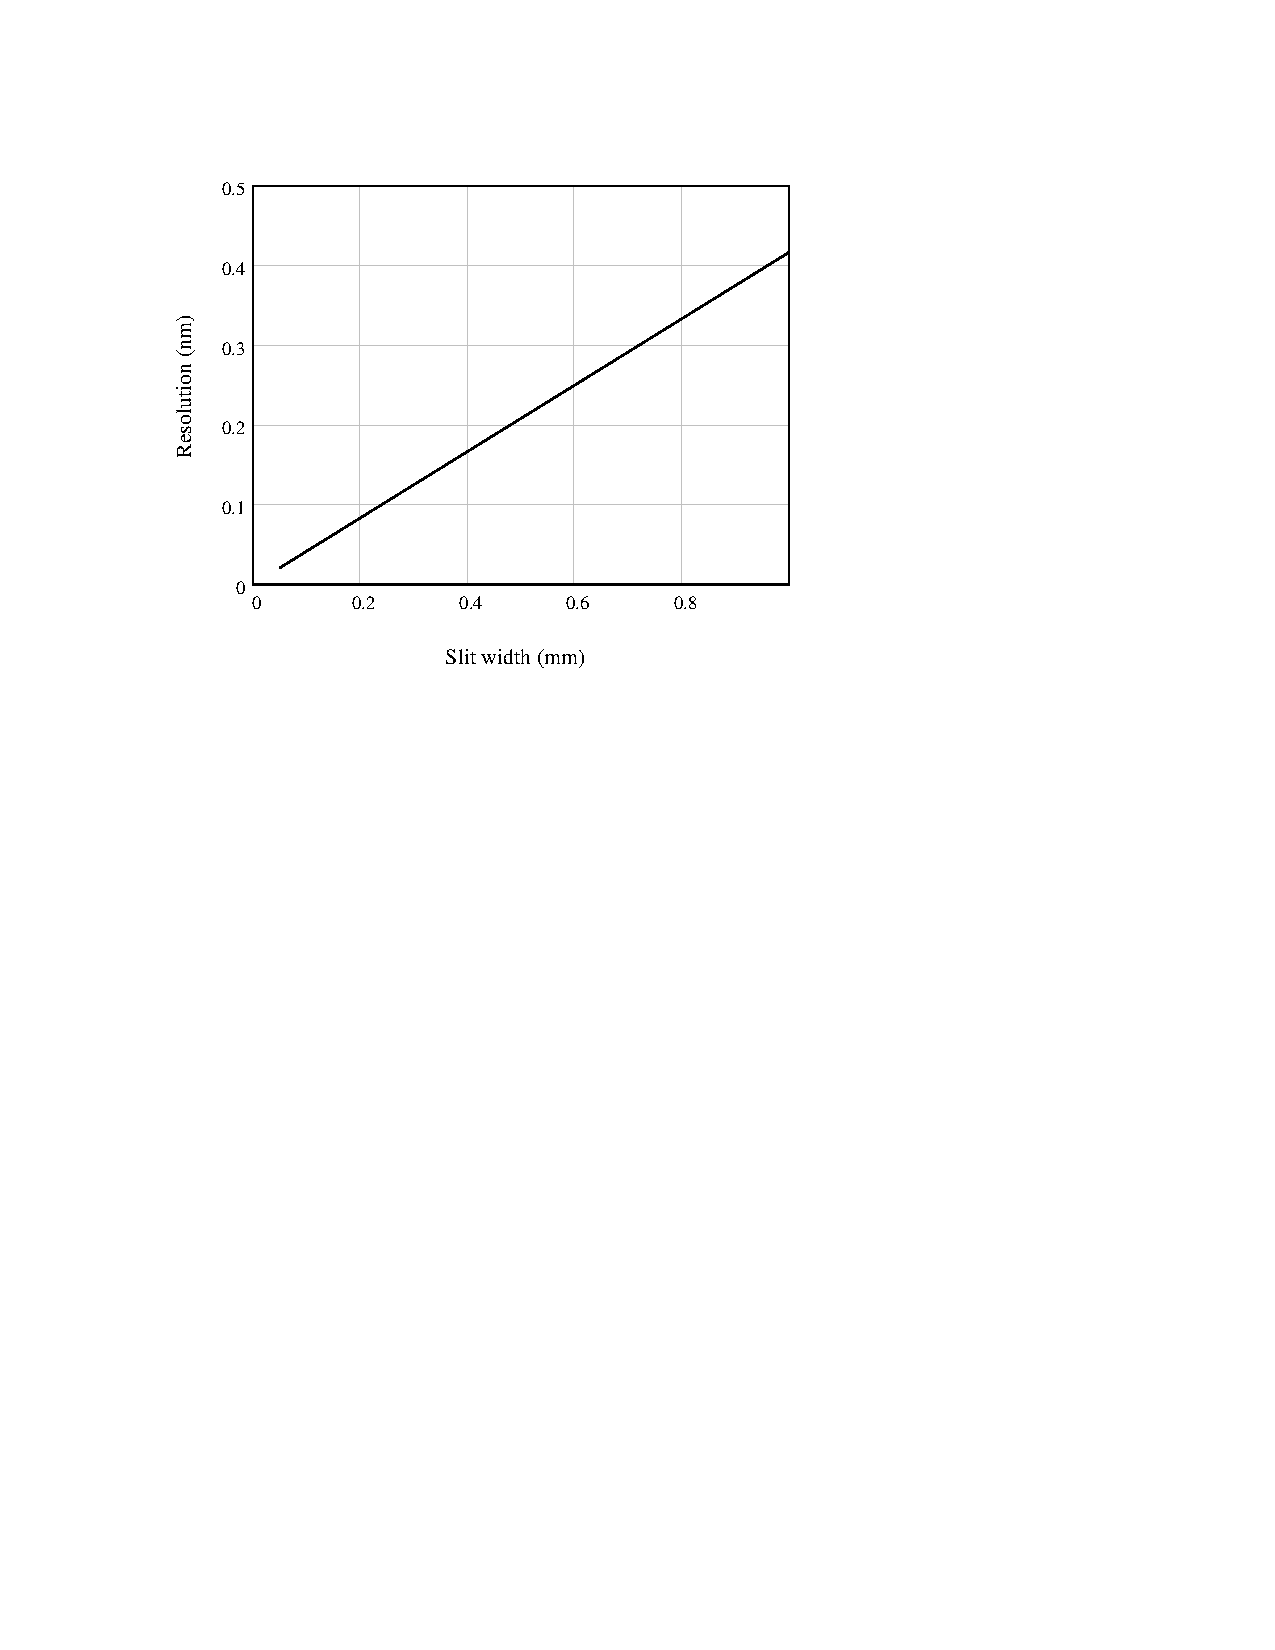
\includegraphics[bb=-30 478 489 700]
{far_nm/far_nm.pdf}
}
\caption[Ideal 1 m monochromator resolution (nm) for large slit widths]{Ideal 1 m monochromator resolution (nm) for large slit widths - Equations \ref{Rayleigh} and \ref{resolvance} imply $\Delta\lambda = a/(2mL\rho)$; here the resolution ($\Delta\lambda$) is ploted for $m=1$, $L=1$ m, and $\rho=1200$ lines per mm.}
\label{far_nm}
\end{figure}
%----------------------------------------------------------------------------

%----------------------------------------------------------------------------
%----------------------------------------------------------------------------
%----------------------------------------------------------------------------
%----------------------------------------------------------------------------
